With the verification of Moltres' neutronics modeling capabilities in the
context of the \gls{MSFR}, we now move on to the multiphysics simulation
results. This chapter covers the steady-state multiphysics simulation results
from Moltres.

The procedure for obtaining the steady-state results involved several steps
due to the highly coupled \glspl{PDE}. First, we ran a preliminary transient
simulation of fluid flow in the \gls{MSFR} core, starting from zero inlet
velocity and gradually ramping it up to match the nominal flow rate (4.5 m$^3$
s$^{-1}$); otherwise Moltres had difficulty converging to the desired fully
developed flow profile. We imposed a parabolic flow profile at the inlet.
Next, we imported these fully developed flow values as initial values for
velocity in the actual transient simulation modeling the full coupled
neutronics and thermal-hydraulics. The initial values for the temperature and
neutron group flux distributions are 953 K and $1 \times 10^{14}$ cm$^{-2}$
s$^{-1}$ uniformly throughout the geometry. Finally, we assume that steady
state is reached when the volume integral values of every variable remain
constant (up to 6 sig. fig.) for at least four seconds in the simulation; this
time period corresponds to the nominal circulation time of the \gls{MSFR}.

For a direct comparison with the steady-state results from the Polimi and
TUDelft models \cite{aufiero_development_2014}, we will first present our
steady-state results without modeling decay heat. After this comparison, we
separately discuss the minor differences borne from decay heat modeling in the
last subsection.

\section{Steady-State Thermal-Hydraulics Results}

\begin{figure}[t!]
    \centering
    \begin{subfigure}[t]{.365\textwidth}
        \centering
        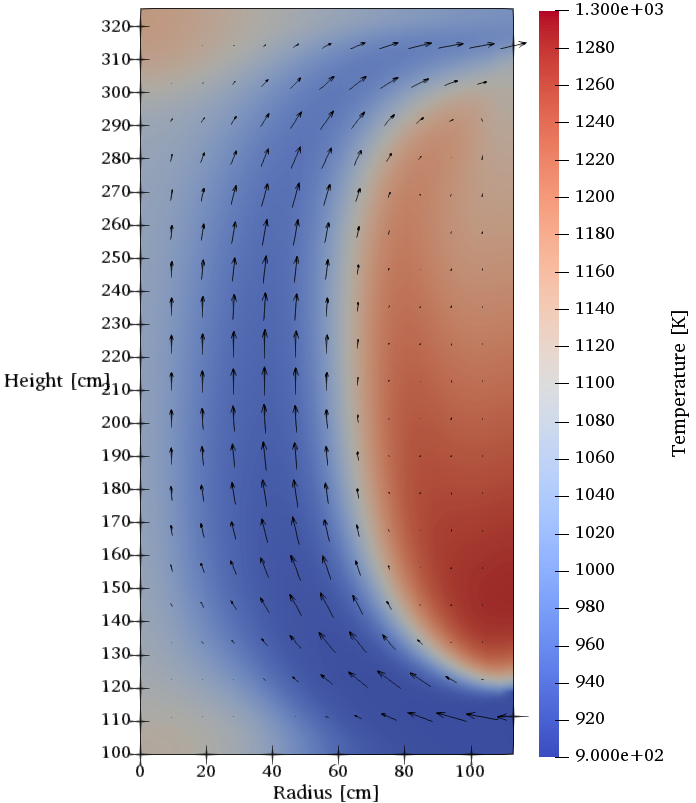
\includegraphics[width=\textwidth]{flow-temp}
    \end{subfigure}
    \hfill
    \begin{subfigure}[t]{.625\textwidth}
        \centering
        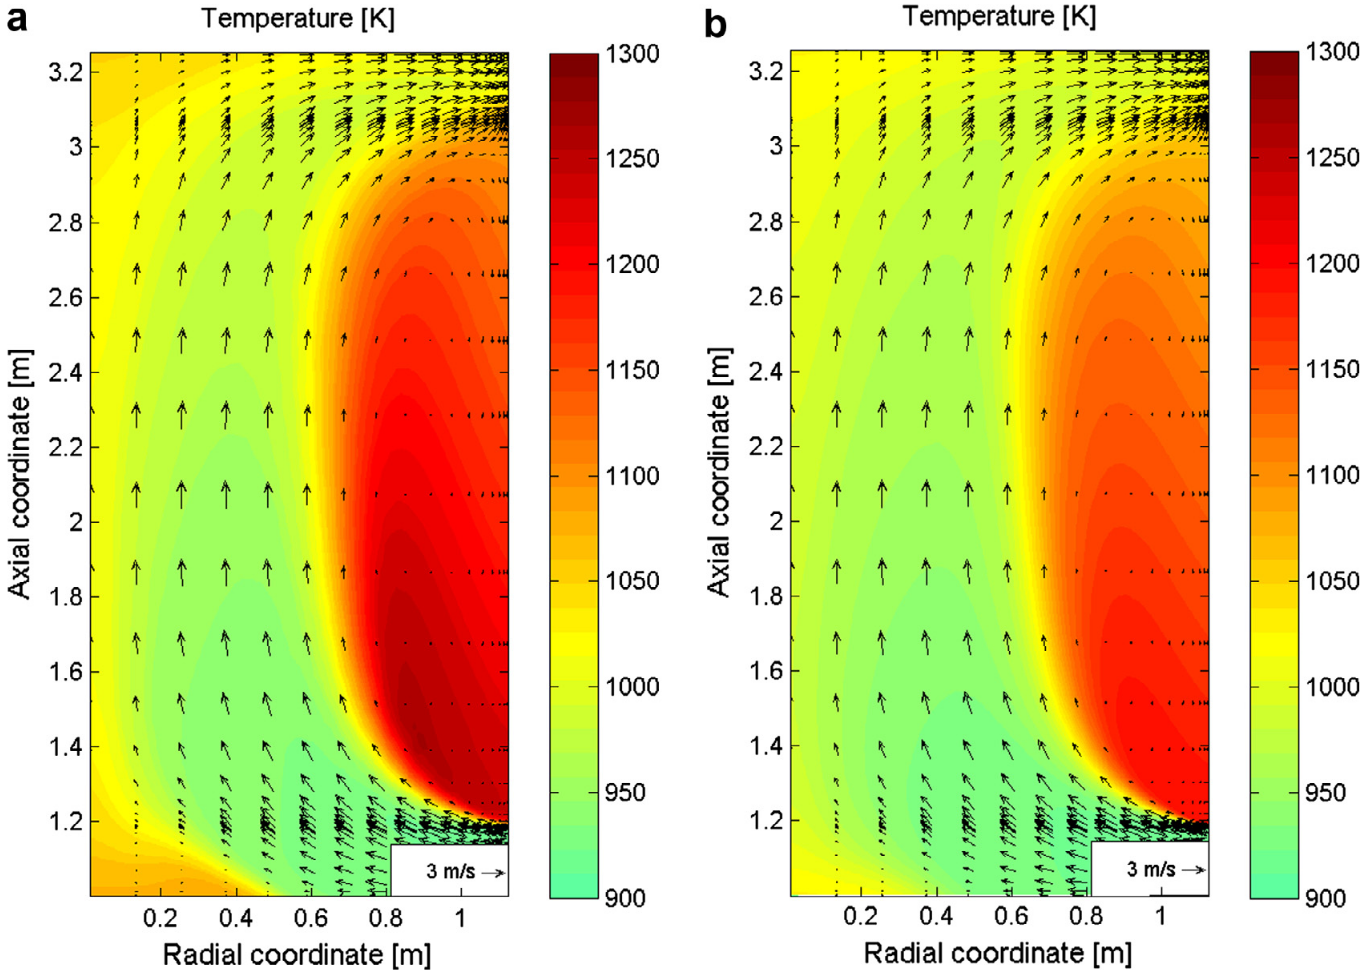
\includegraphics[width=\textwidth]{flow-temp-fiorina}
    \end{subfigure}
    \caption{Temperature and velocity fields in the core from Moltres
    (left), Polimi (center), and TUDelft (right) models. The colors represent
    temperature according to the respective colorbars while the arrows
    represent velocity fields.}
    \label{fig:flow-temp}
\end{figure}

\begin{figure}[t!]
    \centering
    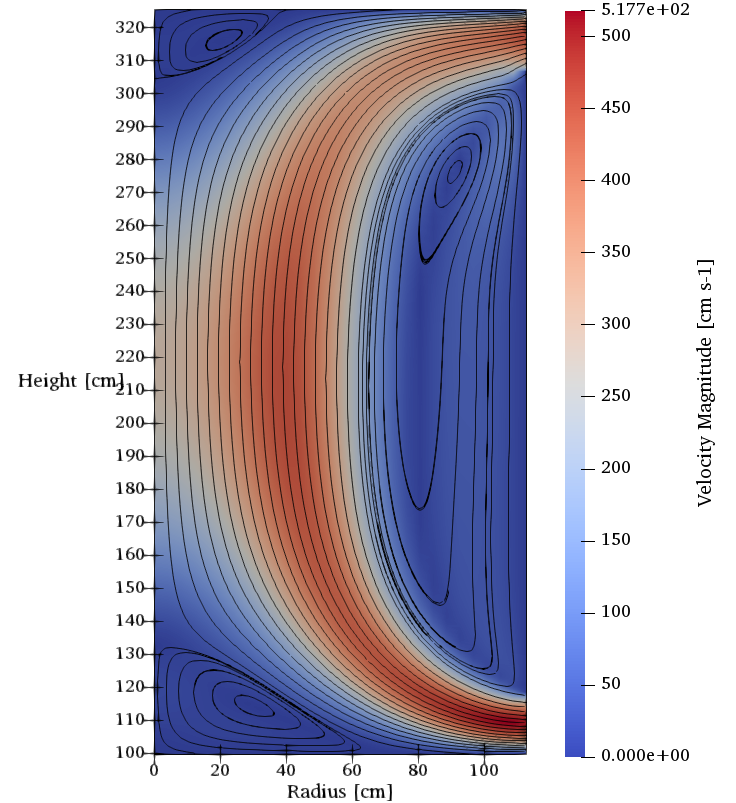
\includegraphics[width=.6\textwidth]{flow}
    \caption{Fuel salt flow streamlines and velocity magnitude in the core.
    The colors represent velocity magnitude according to the colorbar on the
    right.}
    \label{fig:flow}
\end{figure}

Figure \ref{fig:flow-temp} shows the temperature and velocity fields of the
fuel salt in the core at steady state from Moltres and the Polimi and TUDelft
models. Figure \ref{fig:flow} provides an alternate view of the flow profile
through flow streamlines superimposed on the velocity magnitude distribution.
The results from Moltres show good qualitative agreement with the
Polimi and TUDelft models \cite{fiorina_modelling_2014}; we observe similar
flow and hotspot features in all three models. Furthermore, the highest salt
velocities in all three models occur at the inlet, outlet, and at core
half-height approximately 0.40 m away from the central axis. There is a large
recirculation region near the blanket tank walls arising from turbulent flow.
Inertial forces dominate over viscous forces to form this large eddy. The main
difference between Moltres and Fiorina et al.'s models is the flow profile
near the central axis at the top and bottom of the core.
The Polimi and TUDelft models predict relatively stagnant flow in these
regions without recirculation. Moltres, on the other hand, predicts explicit
recirculating flow in these regions. This is due to our constant turbulent
viscosity approximation in Moltres. The k-$\epsilon$ turbulence models in the
Polimi and TUDelft models predict that the turbulent viscosity in these
regions is as high as 100 Pa s, much higher than our 40 Pa s approximation.

Nevertheless, similar temperature hotspots form in these regions of
recirculation and stagnation as convection is the dominant heat transfer
mechanism. The maximum temperature from Moltres, 1275 K near the bottom of the
large recirculation zone, is closer to the maximum temperature in the Polimi
model ($\approx$ 1300 K) than the TUDelft model ($\approx$ 1200K). Similarly,
we observe cooler temperatures in high-velocity regions. The minimum
temperature is 924 K at the inlet. 

While the temperatures at the hotspots are well below the melting point of the
Ni-alloy structure (1500 K), they may cause undue thermal stress on the
blanket tank structure and induce relatively faster salt corrosion rates. A
sudden, large reactivity insertion could push fuel salt temperatures above the
melting point of the Ni-alloy and cause irreversible damage. Furthermore,
the reservoir of hot fuel salt may cause unpredictable behavior during
transient scenarios when the flow profile undergoes a drastic change.
Thus, Rouch et al. \cite{rouch_preliminary_2014} developed an improved
hourglass-shaped design to optimize flow distribution and prevent these
recirculation zones and hotspots from forming. A study of this new design
using Moltres is a potential subject for future work when a proper turbulence
model is in place.

\section{Steady-State Neutronics Results}

\subsection{Neutron Flux}

The neutron flux distribution represents the heat source distribution in a
nuclear reactor. Figure \ref{fig:neutronflux} shows the neutron flux
distributions in the core for all six neutron energy groups, and Figure
\ref{fig:axialradial} shows the axial and radial fluxes along the center of
the core and at reactor half-height, respectively.
The distributions are highly symmetric along the
central and horizontal axes, as expected of a cylindrical reactor design. The
relatively lower temperatures near the center of the core promotes the neutron
flux peaking but it is not a major concern as there are no structural parts
vulnerable to neutron damage in that region. The peak total flux at the center
is $9.80 \times 10^{15}$ cm$^{-2}$ s$^{-1}$, which is close to values reported
by Fiorina et al. \cite{fiorina_molten_2013} and Aufiero et al.
\cite{aufiero_development_2014} as shown in Table \ref{table:peak-flux}. The
peak flux value from this paper is slightly higher as we used the steady-state
temperature distribution while Fiorina et al. and Aufiero et al. imposed a
uniform temperature distribution at 973 K.

\begin{figure}[b!]
    \centering
    \begin{subfigure}[t]{.325\textwidth}
        \centering
        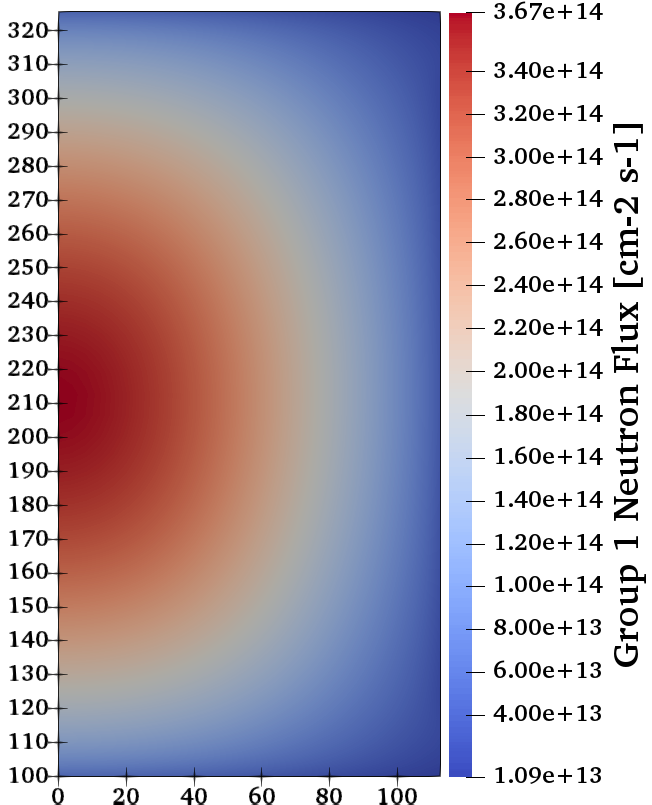
\includegraphics[width=\textwidth]{ss-g1}
    \end{subfigure}
    \begin{subfigure}[t]{.325\textwidth}
        \centering
        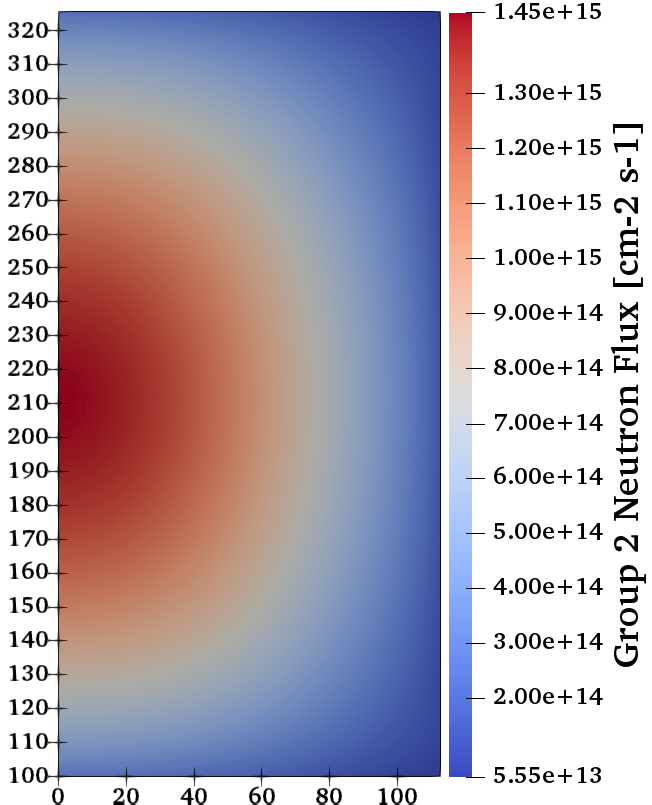
\includegraphics[width=\textwidth]{ss-g2}
    \end{subfigure}
    \begin{subfigure}[t]{.325\textwidth}
        \centering
        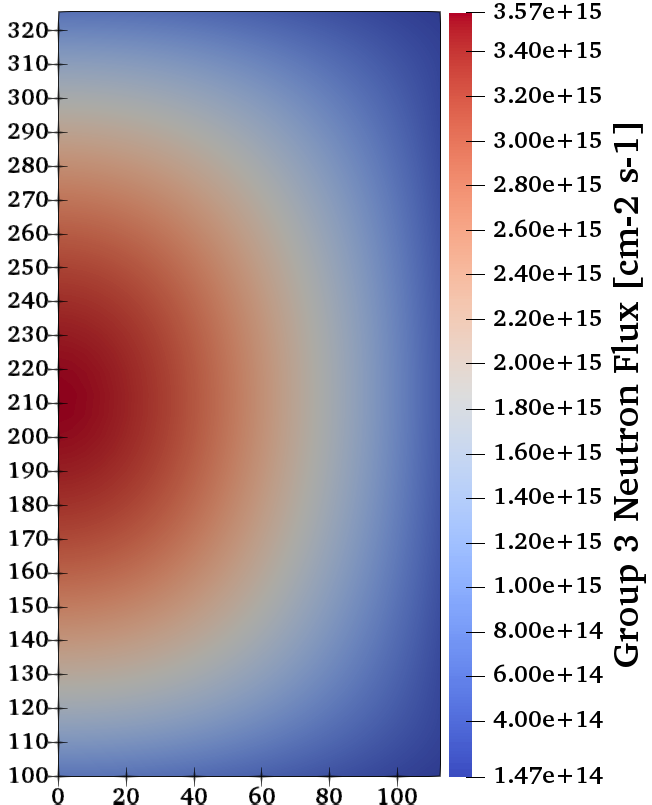
\includegraphics[width=\textwidth]{ss-g3}
    \end{subfigure}
    \begin{subfigure}[t]{.325\textwidth}
        \centering
        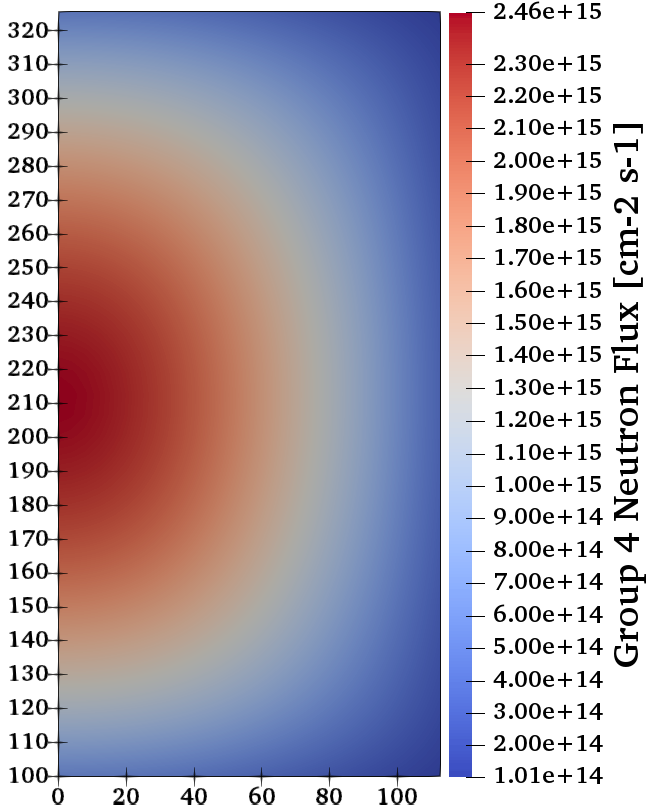
\includegraphics[width=\textwidth]{ss-g4}
    \end{subfigure}
    \begin{subfigure}[t]{.325\textwidth}
        \centering
        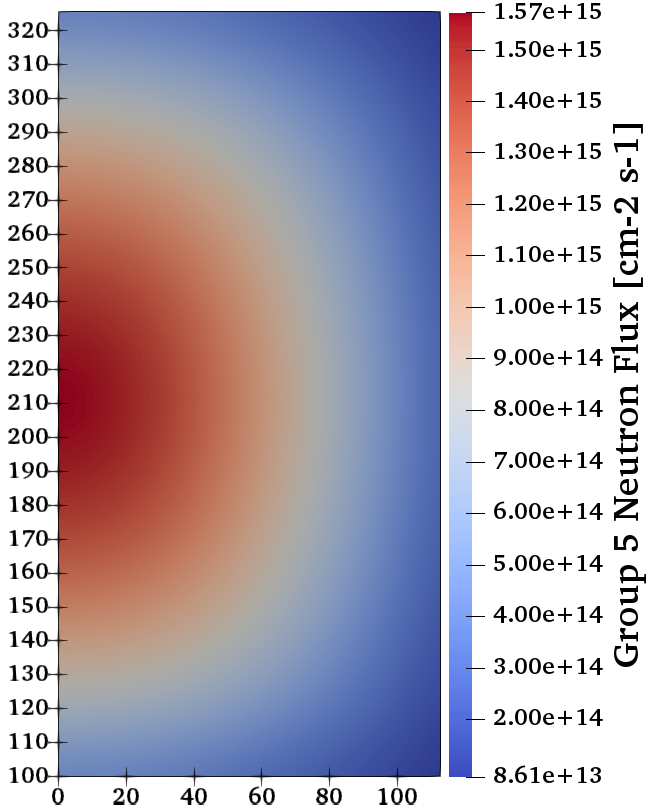
\includegraphics[width=\textwidth]{ss-g5}
    \end{subfigure}
    \begin{subfigure}[t]{.325\textwidth}
        \centering
        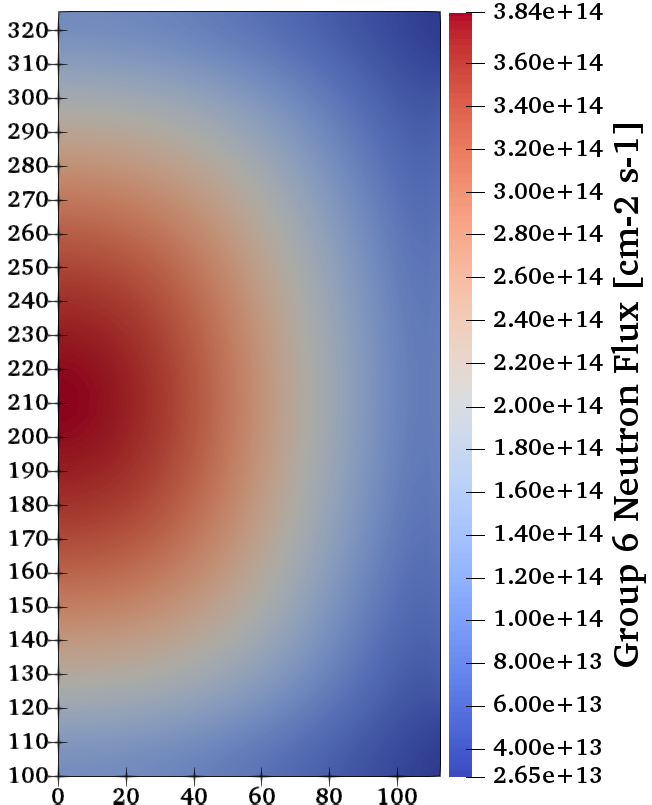
\includegraphics[width=\textwidth]{ss-g6}
    \end{subfigure}
    \caption{Neutron flux distributions in the core for neutron energy groups
    1 to 6. The y and x axes represent height and radius (in cm) of the core
    relative to the entire reactor geometry.}
    \label{fig:neutronflux}
\end{figure}

\begin{figure}[t!]
    \centering
    \begin{subfigure}[t]{.49\textwidth}
        \centering
        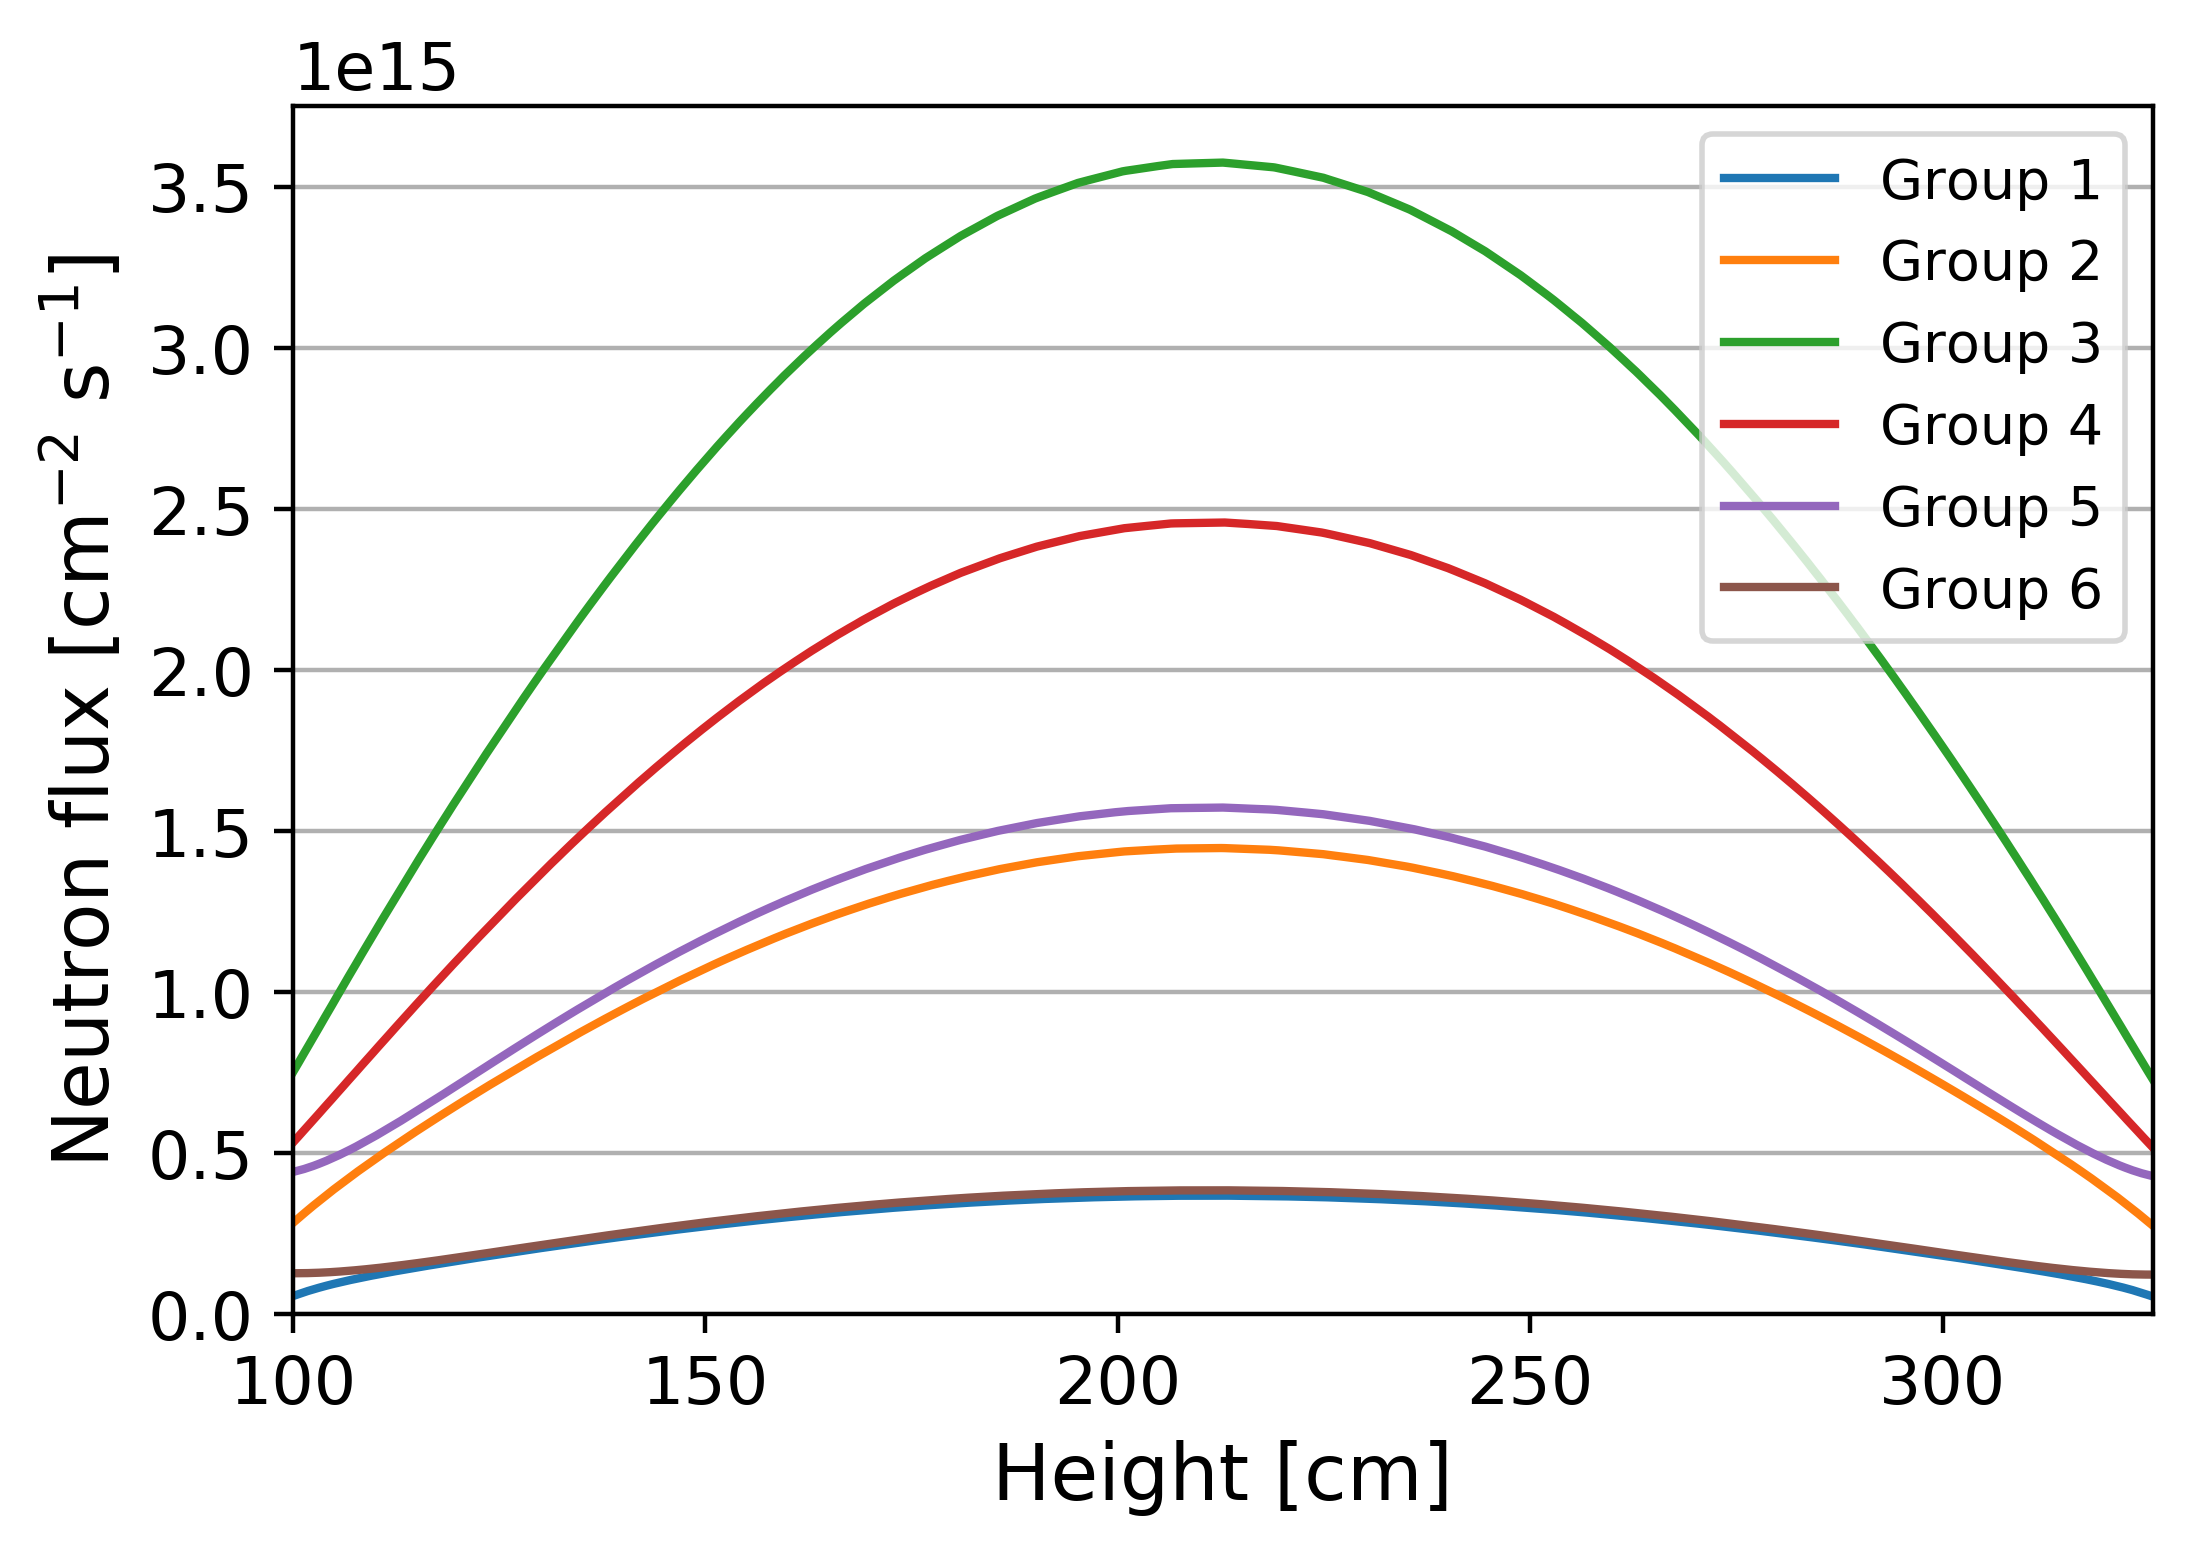
\includegraphics[width=\textwidth]{axial-flux}
    \end{subfigure}
    \begin{subfigure}[t]{.49\textwidth}
        \centering
        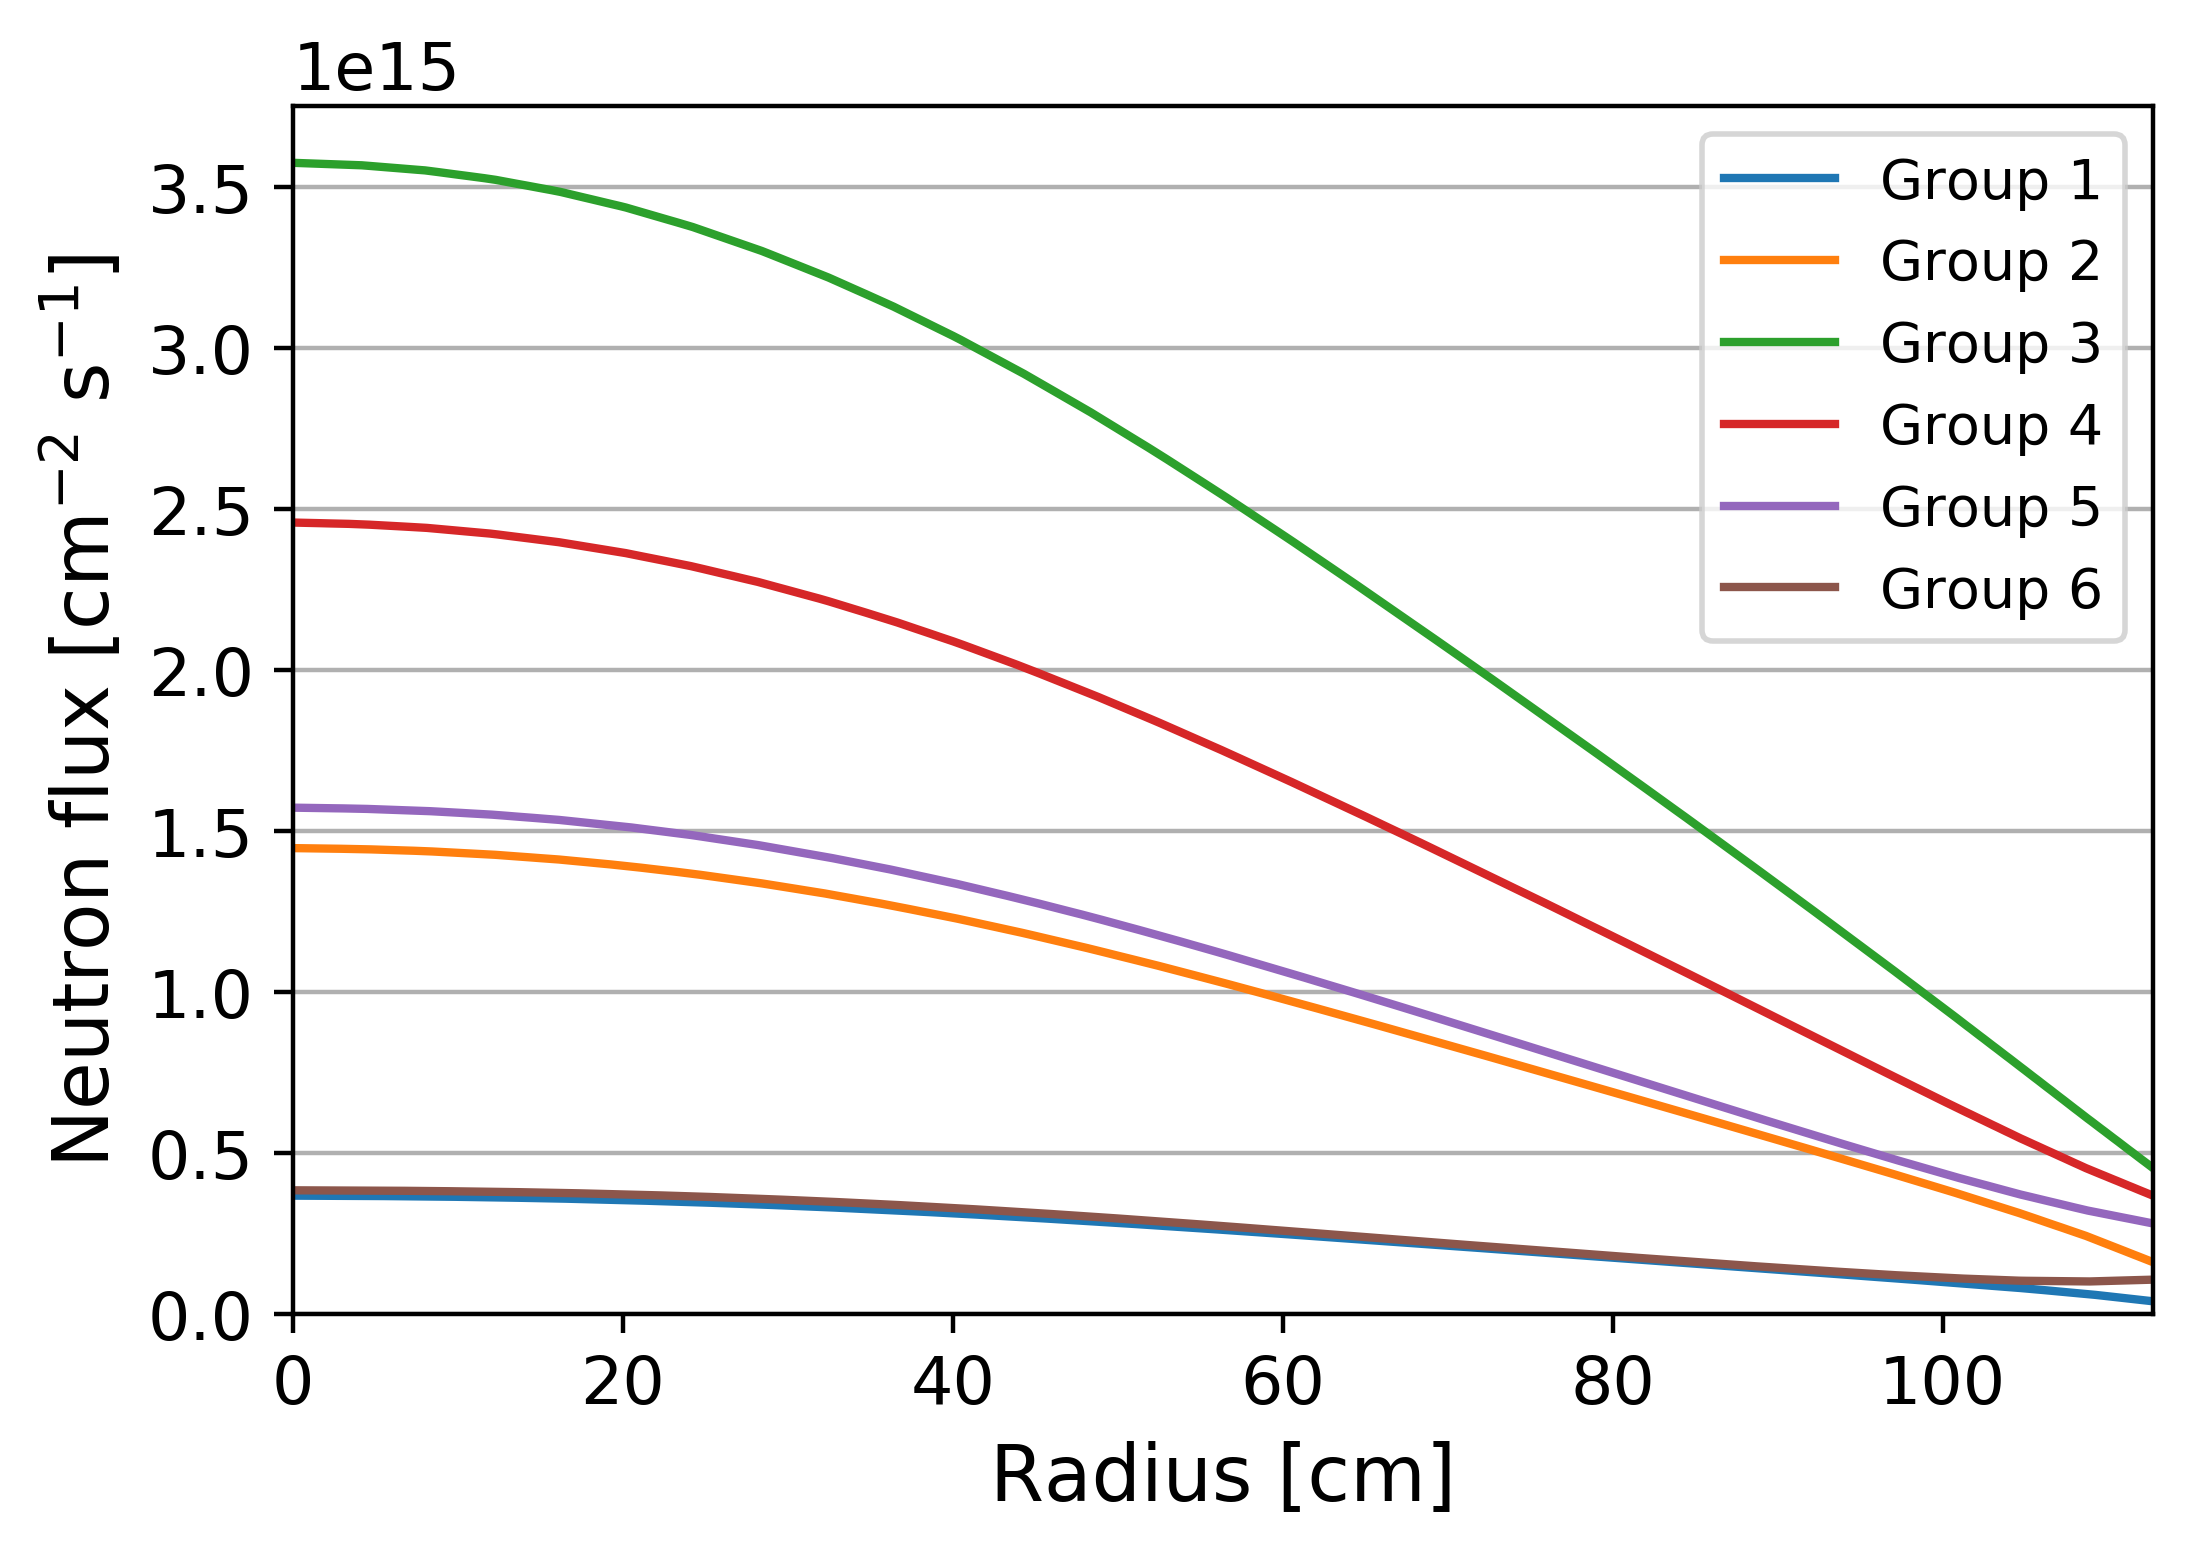
\includegraphics[width=\textwidth]{radial-flux}
    \end{subfigure}
    \caption{Axial (left) and radial (right) neutron flux distributions in the
    core for neutron energy groups 1 to 6.}
    \label{fig:axialradial}
\end{figure}

\begin{table}[b!]
	\centering
	\caption{Peak neutron flux values from Moltres (this paper), COMSOL
	\cite{fiorina_molten_2013}, and OpenFOAM \cite{aufiero_development_2014}
	models along with the temperature distribution with which the values were
	obtained.}
	\begin{tabular}{l l S}
		\toprule
		{Model} & {Temperature distribution} & {Peak Neutron Flux [$\times 10^{15}$ cm$^{-2}$ s$^{-1}$]}
		\\
		\midrule
		{Moltres (This paper)} & {Steady state} & 9.80\\
		{COMSOL} & {Uniform, 973 K} & 8.6 \\
		{OpenFOAM} & {Uniform, 973 K} & 9.0 \\
		\bottomrule
	\end{tabular}
	\label{table:peak-flux}
\end{table}

\begin{figure}[t!]
    \centering
    \begin{subfigure}[t]{.243\textwidth}
        \centering
        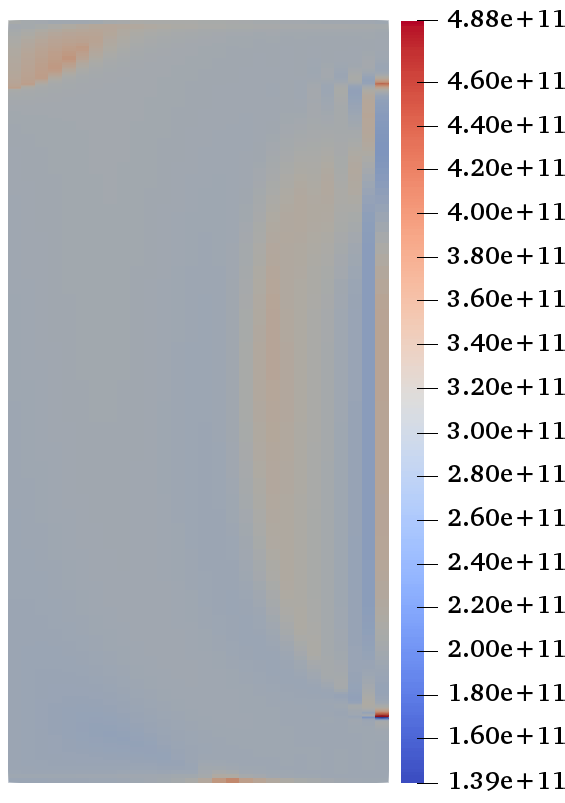
\includegraphics[width=\textwidth]{ss-pre1}
    \end{subfigure}
    \begin{subfigure}[t]{.243\textwidth}
        \centering
        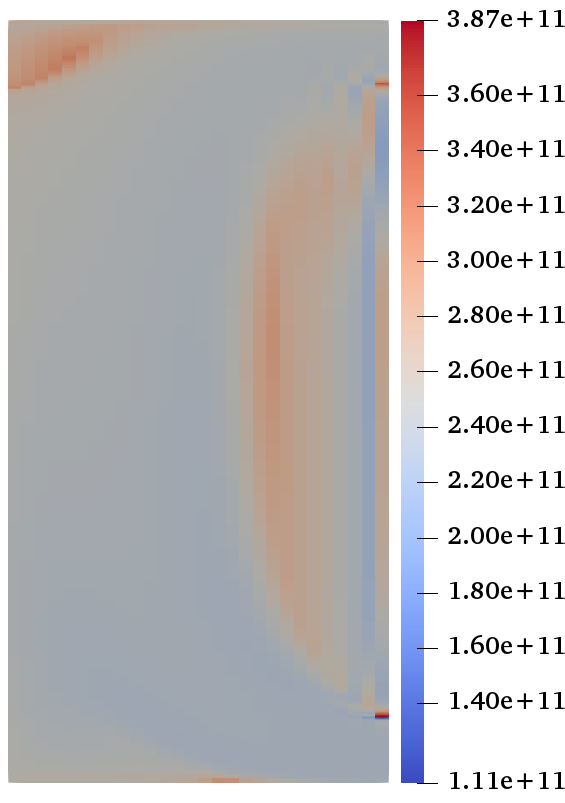
\includegraphics[width=\textwidth]{ss-pre2}
    \end{subfigure}
    \begin{subfigure}[t]{.243\textwidth}
        \centering
        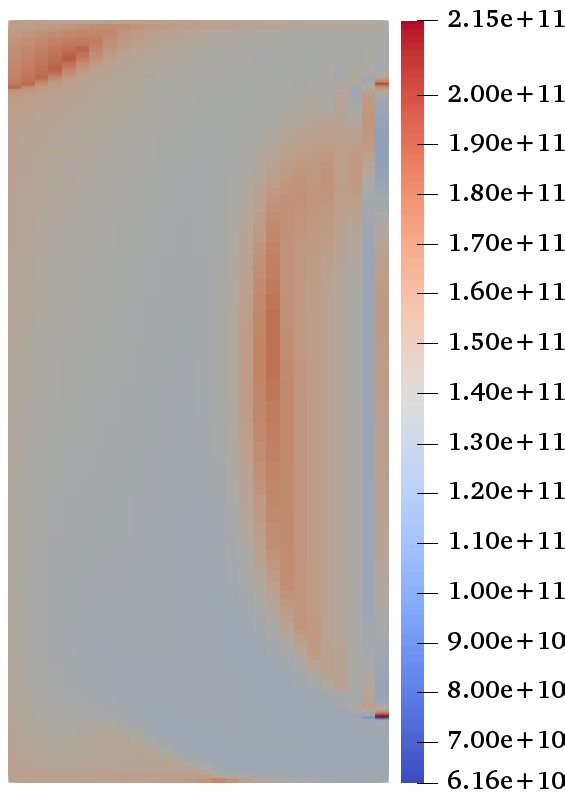
\includegraphics[width=\textwidth]{ss-pre3}
    \end{subfigure}
    \begin{subfigure}[t]{.243\textwidth}
        \centering
        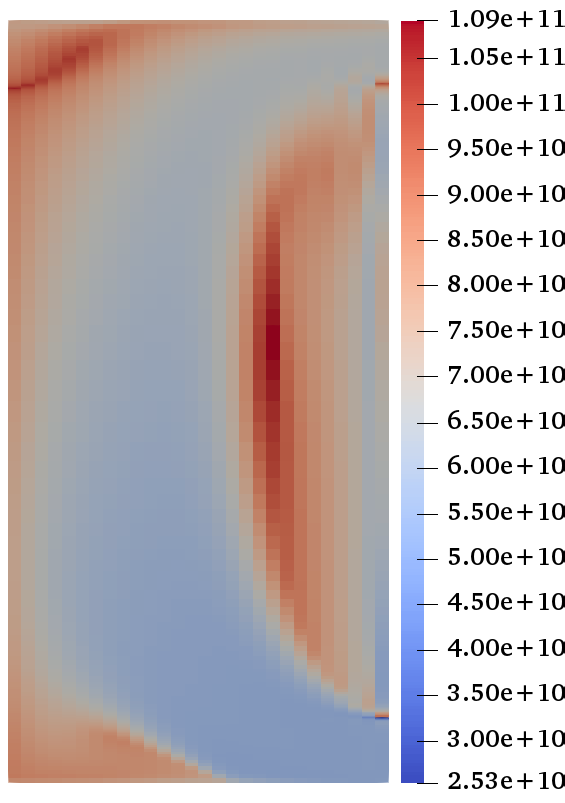
\includegraphics[width=\textwidth]{ss-pre4}
    \end{subfigure}
    \begin{subfigure}[t]{.243\textwidth}
        \centering
        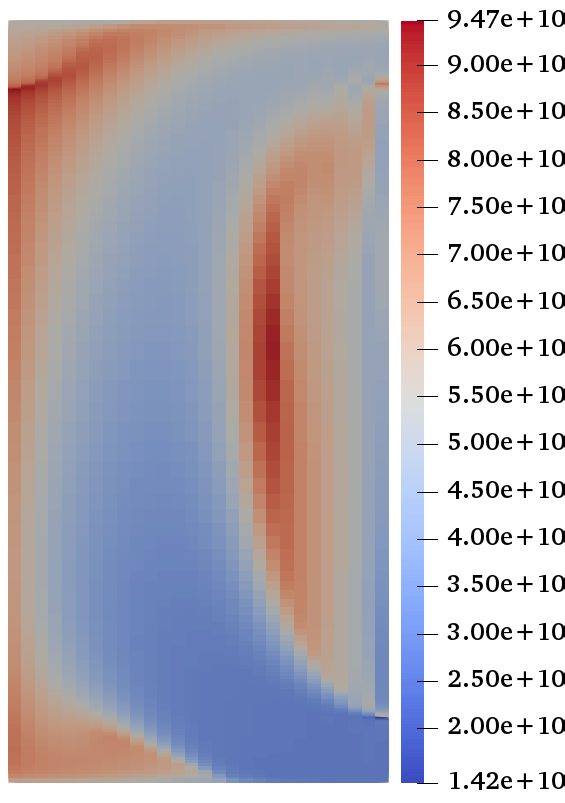
\includegraphics[width=\textwidth]{ss-pre5}
    \end{subfigure}
    \begin{subfigure}[t]{.243\textwidth}
        \centering
        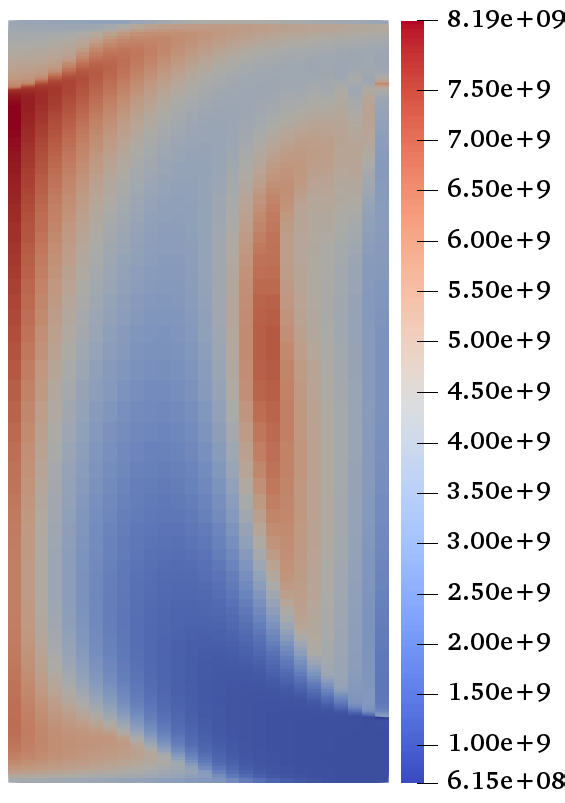
\includegraphics[width=\textwidth]{ss-pre6}
    \end{subfigure}
    \begin{subfigure}[t]{.243\textwidth}
        \centering
        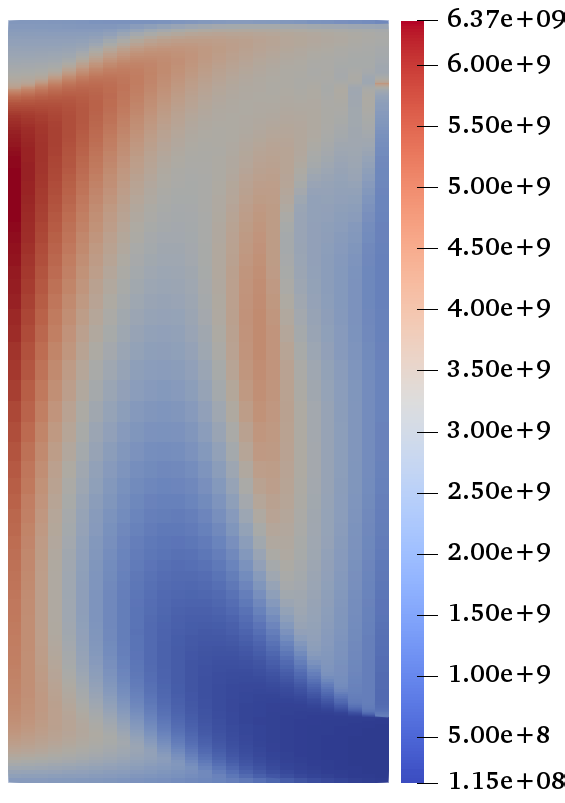
\includegraphics[width=\textwidth]{ss-pre7}
    \end{subfigure}
    \begin{subfigure}[t]{.243\textwidth}
        \centering
        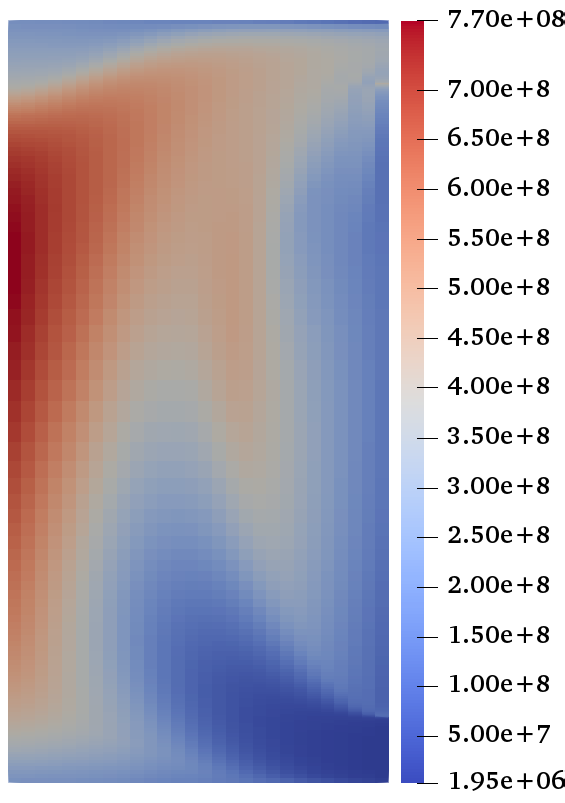
\includegraphics[width=\textwidth]{ss-pre8}
    \end{subfigure}
    \caption{\gls{DNP} distributions in the core for \gls{DNP} groups
    1 to 8 (from left to right, top to bottom). Refer to Figure \ref{fig:neutronflux} for the height and radius
    scales on the y and x axes, respectively. Note the different scales for
    each distribution.}
    \label{fig:dnp}
\end{figure}

\subsection{Delayed Neutron Fraction}

As mentioned earlier, the delayed neutron precursors (DNPs) are mobile in
\glspl{MSR} and their distributions do not directly correspond to the neutron
flux distributions. The location where the \glspl{DNP} decay and emit neutrons
impacts their neutron
importance depending on their proximity to fissile and parasitic isotopes.
Figure \ref{fig:dnp} shows the \gls{DNP} distributions for all eight \gls{DNP}
groups. In general, we observe less \glspl{DNP} in the regions with fast salt
flow, namely
 The
precursors from the shortest-lived group (Group 8) predominantly decay within
the core as their half-lives are shorter than the time it takes to reach the
outlet while the precursors from the longest-lived group (Group 1) are
relatively evenly distributed due to their long half-lives. For the
longer-lived groups, the \gls{DNP} concentrations are not well-resolved on the
mesh elements adjacent to the outlet and the inlet boundaries, respectively.
Thus, we recommend careful mesh refinement for future work involving similar
geometries.

\begin{figure}[b!]
    \centering
    \begin{subfigure}[t]{.30\textwidth}
        \centering
        \vspace{.9cm}
        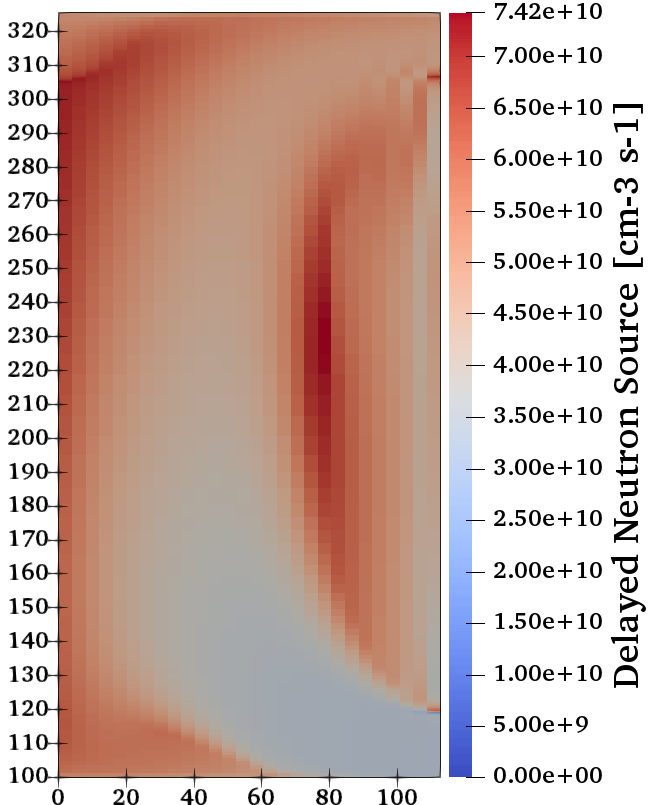
\includegraphics[width=\textwidth]{ss-pre}
    \end{subfigure}
    \begin{subfigure}[t]{.69\textwidth}
        \centering
        \vspace{0pt}
        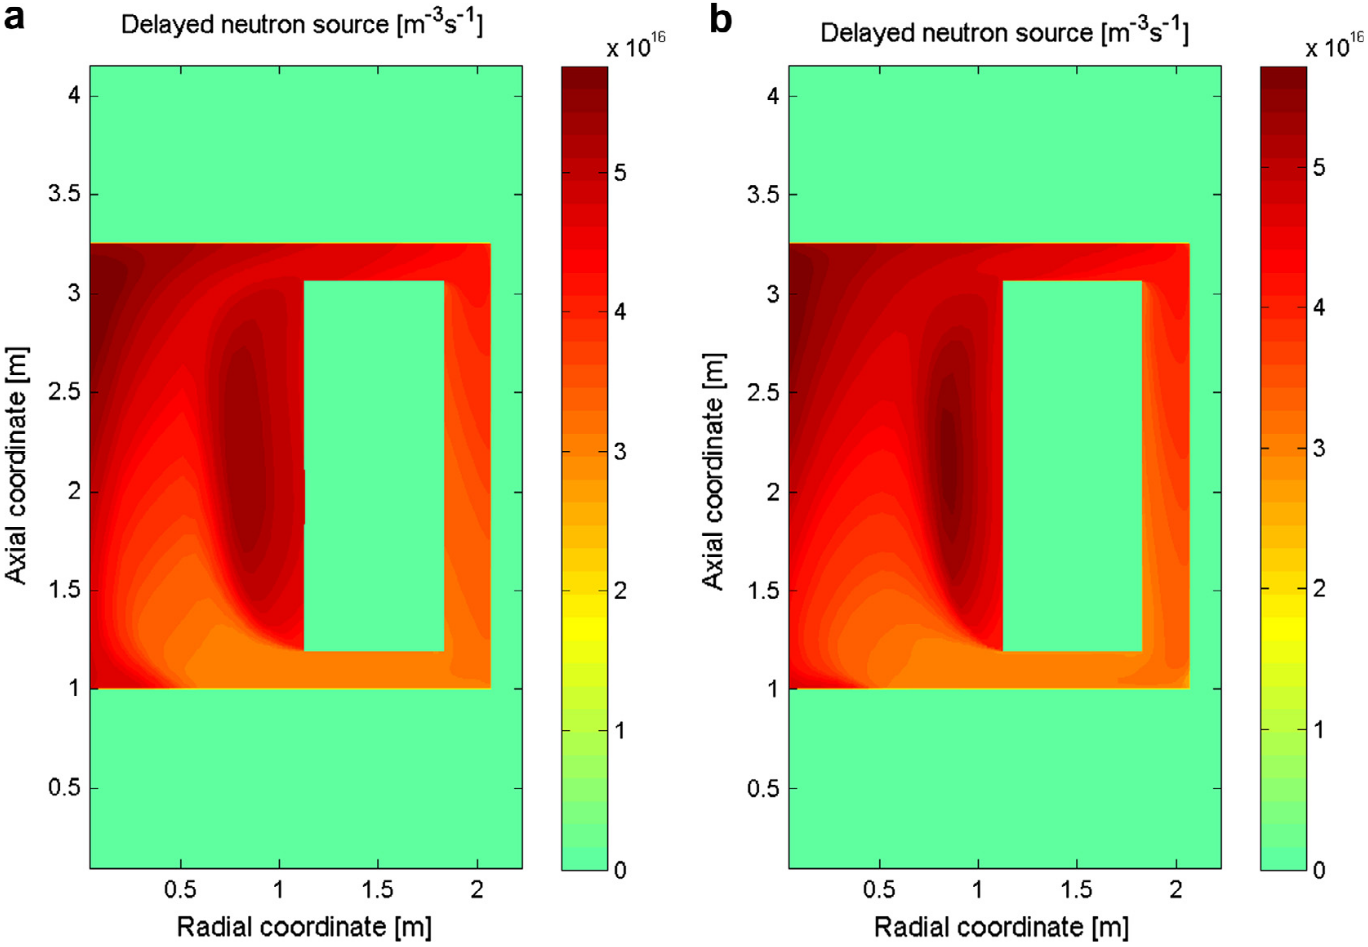
\includegraphics[width=\textwidth]{fiorina-pre}
    \end{subfigure}
    \caption{Total \gls{DNP} distribution in the core from Moltres
    (left), Polimi (center), and TUDelft (right) models.}
    \label{fig:pre}
\end{figure}

In Figure \ref{fig:pre}, we compare the total delayed neutron source
distribution from Moltres with the results from the Polimi and TUDelft models
\cite{fiorina_modelling_2014}. In contrast to Figure \ref{fig:dnp} which shows
the precursor distribution, Figure \ref{fig:pre} shows the rate of delayed
neutron emission, which we calculated by multiplying each \gls{DNP} group
$C_i$ with its associated decay constant $\lambda_i$.
We observe that the Polimi and TUDelft models
feature greater \gls{DNP} retention in the stagnant regions within the core.
This effect is less pronounced in the Moltres model. There is less build-up
of \glspl{DNP} at the top of the core in Moltres because most of the
\glspl{DNP} produced near the center of the core cannot enter the axial
recirculation zone that only appears in Moltres. We also observe less build-up
in the large recirculation zone near the blanket tank.

The in-core delayed neutron fraction $\beta_c$ is an important safety
parameter for \glspl{MSR}. This value represents the actual delayed
neutron fraction in \glspl{MSR} after accounting for the loss of delayed
neutrons from \glspl{DNP} decaying outside the active core region. In general,
reactors with smaller $\beta$ values exhibit greater prompt jumps in the
neutron flux in response to reactivity insertions because they have a greater
proportion of prompt neutrons under normal operating conditions. This is
undesirable from a reactor safety perspective because it exposes the reactor
to relatively more extreme conditions before active safety mechanisms
activate and scram the reactor. In \glspl{MSR}, this danger is partly
mitigated by the strong, negative fuel temperature reactivity coefficient. 
Chapter 6 contains more in-depth discussions for various transient scenarios.

In Table \ref{table:dnf}, we compare the fraction of out-of-core emissions and
the $\beta_c$ values from Moltres with the Polimi and TUDelft models. We
calculated the fraction of out-of-core emissions by finding the total amount
of each \gls{DNP} group in the core and the outer loop, multiplying each total
by their associated decay time constants $\lambda_i$, and calculating the
proportion of emissions in the outer loop relative to the grand total. We
calculated $\beta_c$ by first obtaining the prompt neutron emission rate from
Moltres and subsequently using in-core delayed neutron emission rate from the
previous calculation to find the fraction of delayed neutron emission rate
relative to total emission rate.

\begin{table}[t!]
	\centering
	\caption{The fraction of delayed neutrons lost from out-of-core emission
	and the in-core delayed neutron fraction $\beta_c$ values from Moltres
	(this paper), and the Polimi and TUDelft models
	\cite{fiorina_modelling_2014}.}
	\begin{tabular}{l S S}
		\toprule
		{Model} & {Out-of-Core Emission [\%]} & {$\beta_c$ [pcm]}
		\\
		\midrule
		{Moltres (This paper)} & {44.16} & {184.9}\\
		{Polimi} & {34.80} & {134.3} \\
		{TUDelft} & {34.85} & {123.8} \\
		\bottomrule
	\end{tabular}
	\label{table:dnf}
\end{table}

The fraction of out-of-core emissions from our Moltres model
differs significantly by approximately 10\%, while $\beta_c$ differs by
60-70 pcm. We attribute the former to the lesser \gls{DNP} retention in the
stagnant flow regions in the core; the \glspl{DNP} are more evenly distributed
along the entire primary loop, leading to more delayed neutron emissions in
the outer loop region. The most likely reason for this is differences in the
flow pattern in the recirculation zone because convective species transport
dominates diffusive effects in the \gls{MSFR}. The exact flow pattern in the
recirculation zones in the Polimi and TUDelft models is likely to differ from
that in Moltres (Figure \ref{fig:flow}). Figure \ref{fig:flow-temp} also shows
some minor differences in the magnitude of the flow in the recirculation zones
between Moltres, and the Polimi and TUDelft models. Although the sizes of the
arrows representing flow velocity are not normalized to the same scales, a
quick comparison between the largest arrows and the arrows in the
recirculation zone indicate that the recirculation zone in Moltres is
relatively more stagnant. This could explain the concentration of \glspl{DNP}
along an ``arc'' closer to the center of the core in Moltres as opposed to the
more even distribution of \glspl{DNP} throughout the whole recirculation zones
in the Polimi and TUDelft models. The higher peak \glspl{DNP} distribution in
Moltres also supports this assertion.

In spite of the greater delayed neutron losses, the $\beta_c$ value is higher
in Moltres than the Polimi and TUDelft models. To account for this
peculiarity, we note that Fiorina et al. \cite{fiorina_modelling_2014}
applied adjoint flux weighting for their $\beta_c$ calculation while we report
our value as the physical fraction without adjoint weighting. The weighting
results in a significant difference in $\beta_c$ because a large fraction of
the \glspl{DNP} decay in the recirculation zones, where the neutron importance
is noticeably diminished.

\section{Decay Heat}

The inclusion of a decay heat model effectively redistributes a fraction of
the volumetric heat source from the center of the core to the entire loop.
Thus, we expect to observe a slight flattening of the temperature distribution
across the entire primary loop.
